% Sablon pentru realizarea lucrarii de licenta, conform cu recomandarile
% din ghidul de redactare:
% - https://fmi.unibuc.ro/finalizare-studii/
% - https://drive.google.com/file/d/1xj9kZZgTkcKMJkMLRuoYRgLQ1O8CX0mv/view

% Multumiri lui Gabriel Majeri, acest sablon a fost creat pe baza
% codului sursa a lucrarii sale de licenta. 
% Codul sursa: https://github.com/GabrielMajeri/bachelors-thesis
% Website: https://www.gabrielmajeri.ro/
%
% Aceast sablon este licentiat sub Creative Commons Attribution 4.0 International License.

\documentclass[12pt, a4paper]{report}

\usepackage{tgtermes} % times font

% Suport pentru diacritice și alte simboluri
\usepackage{fontspec}

% Suport pentru mai multe limbi
\usepackage{polyglossia}

% Setează limba textului la română
\setdefaultlanguage{romanian}
% Am nevoie de engleză pentru rezumat
\setotherlanguages{english}

% Indentează și primul paragraf al fiecărei noi secțiuni
\SetLanguageKeys{romanian}{indentfirst=true}

% Suport pentru diferite stiluri de ghilimele
\usepackage{csquotes}

\DeclareQuoteStyle{romanian}
  {\quotedblbase}
  {\textquotedblright}
  {\guillemotleft}
  {\guillemotright}

% Utilizează biblatex pentru referințe bibliografice
\usepackage[
    maxbibnames=50,
    sorting=nty,
    style=authoryear-comp
]{biblatex}

\addbibresource{bibliografie/bibliography.bib}

% Setează spațiere inter-linie la 1.5
\usepackage{setspace}
\onehalfspacing

% Modificarea geometriei paginii
\usepackage{geometry}

% Include funcțiile de grafică
\usepackage{graphicx}
% Încarcă imaginile din directorul `images`
\graphicspath{{./images/}}

% Listări de cod
\usepackage[svgnames]{xcolor}
  \definecolor{diffstart}{named}{Grey}
  \definecolor{diffincl}{named}{Green}
  \definecolor{diffrem}{named}{OrangeRed}

\usepackage{listings}
  \lstdefinelanguage{diff}{
    basicstyle=\ttfamily\small,
    morecomment=[f][\color{diffstart}]{@@},
    morecomment=[f][\color{diffincl}]{+\ },
    morecomment=[f][\color{diffrem}]{-\ },
  }

\lstdefinestyle{mystyle}{ % Listing design
    basicstyle=\ttfamily\footnotesize,
    breakatwhitespace=false,         
    breaklines=true,                 
    captionpos=b,                    
    keepspaces=true,                 
    %numbers=left,                    
    numbersep=5pt,                  
    showspaces=false,                
    keywordstyle=\bfseries,
    showstringspaces=false,
    escapeinside={(*}{*)},
    showtabs=false,                  
    tabsize=2
}

\lstset{style=mystyle}

% Linkuri interactive în PDF
\usepackage[
    colorlinks,
    linkcolor={black},
    menucolor={black},
    citecolor={black},
    urlcolor={blue}
]{hyperref}

% Simboluri matematice codificate Unicode
\usepackage[warnings-off={mathtools-colon,mathtools-overbracket}]{unicode-math}

% Comenzi matematice
\usepackage{amsmath}
\usepackage{mathtools}

% Formule matematice
\newcommand{\bigO}[1]{\symcal{O}\left(#1\right)}
\DeclarePairedDelimiter\abs{\lvert}{\rvert}

% Suport pentru rezumat în două limbi
% Bazat pe https://tex.stackexchange.com/a/70818
\newenvironment{abstractpage}
  {\cleardoublepage\thispagestyle{empty}}
  {\vfill\cleardoublepage}
\renewenvironment{abstract}[1]
  {\smallskip\selectlanguage{#1}%
   \begin{center}\bfseries\abstractname\end{center}}
  {\par\smallskip}

% Suport pentru anexe
\usepackage[toc]{appendix}
\renewcommand{\appendixtocname}{Anexe}

% Suport pentru abrevieri
\usepackage[acronym]{glossaries}

\makeglossaries
\glstoctrue
\newacronym{iot}{IoT}{Internet of Things}
\newacronym{eda}{EDA}{Event-Driven Architecture}
\newacronym{edas}{EDAs}{Event-Driven Architectures}
\newacronym{p2p}{P2P}{Peer-to-Peer}
\newacronym{qa}{QA}{Quality Assurance}
\newacronym{rfid}{RFID}{Radio-Frequency Identification}
\newacronym{osi}{OSI}{Open Systems Interconnection}
\newacronym{smt}{SMT}{Satisfiability Modulo Theories}

% Suport pentru citate
\usepackage{dirtytalk}

% Stiluri diferite de headere și footere
\usepackage{fancyhdr}

\fancypagestyle{front}{
  \fancyhf{}
  \renewcommand{\headrulewidth}{0pt}
  \cfoot{}
}
\fancypagestyle{main}{
  \fancyhf{}
  \renewcommand\headrulewidth{0pt}
  \fancyhead[C]{}
  \fancyfoot[C]{\thepage}
}

% Metadate
\title{O analiză comparativă a metodelor de testare pentru sistemele Internet-of-Things}
\author{Mihail Feraru}

% Generează variabilele cu @
\makeatletter

\begin{document}

% Front matter
\cleardoublepage
\pagestyle{front}
\let\ps@plain\ps@front

% Pagina de titlu
\begin{titlepage}

% Redu marginile
\newgeometry{left=2cm,right=2cm,bottom=1cm}

\begin{figure}[!htb]
    \centering
    \begin{minipage}{0.2\textwidth}
        
\includegraphics[width=\linewidth]{logo-ub.png}
    \end{minipage}
    \begin{minipage}{0.5\textwidth}
        \large
        \vspace{0.2cm}
        \begin{center}
            \textbf{UNIVERSITATEA DIN BUCUREȘTI}
        \end{center}
        \vspace{0.3cm}
        \begin{center}
            \textbf{
                FACULTATEA DE \\
                MATEMATICĂ ȘI INFORMATICĂ
            }
        \end{center}
    \end{minipage}
    \begin{minipage}{0.2\textwidth}
        
\includegraphics[width=\linewidth]{logo-fmi.png}
    \end{minipage}
\end{figure}

\begin{center}
\textbf{SPECIALIZAREA INFORMATICĂ}
\end{center}

\vspace{1cm}

\begin{center}
\Large \textbf{Lucrare de licență}
\end{center}

\begin{center}
\huge \textbf{\MakeUppercase{\@title}}
\end{center}

\vspace{3cm}

\begin{center}
\large \textbf{Absolvent \\ \@author}
\end{center}

\vspace{0.25cm}

\begin{center}
\large \textbf{Coordonator științific \\ Prof. dr. habil. Alin Ștefănescu}
\end{center}

\vspace{2cm}

\begin{center}
\Large \textbf{București, iunie 2022}
\end{center}
\end{titlepage}

\restoregeometry
\newgeometry{
    margin=2.5cm
}

\addtocounter{page}{1}

% Rezumatul
\begin{abstractpage}

\begin{abstract}{romanian}
Lorem ipsum dolor sit amet, consectetur adipiscing elit. Fusce vitae eros sit amet sem ornare varius. Duis eget felis eget risus posuere luctus. Integer odio metus, eleifend at nunc vitae, rutrum fermentum leo. Quisque rutrum vitae risus nec porta. Nunc eu orci euismod, ornare risus at, accumsan augue. Ut tincidunt pharetra convallis. Maecenas ut pretium ex. Morbi tellus dui, viverra quis augue at, tincidunt hendrerit orci. Lorem ipsum dolor sit amet, consectetur adipiscing elit. Aliquam quis sollicitudin nunc. Sed sollicitudin purus dapibus mi fringilla, nec tincidunt nunc eleifend. Nam ut molestie erat. Integer eros dolor, viverra quis massa at, auctor.
\end{abstract}

\begin{abstract}{english}
Lorem ipsum dolor sit amet, consectetur adipiscing elit. Fusce vitae eros sit amet sem ornare varius. Duis eget felis eget risus posuere luctus. Integer odio metus, eleifend at nunc vitae, rutrum fermentum leo. Quisque rutrum vitae risus nec porta. Nunc eu orci euismod, ornare risus at, accumsan augue. Ut tincidunt pharetra convallis. Maecenas ut pretium ex. Morbi tellus dui, viverra quis augue at, tincidunt hendrerit orci. Lorem ipsum dolor sit amet, consectetur adipiscing elit. Aliquam quis sollicitudin nunc. Sed sollicitudin purus dapibus mi fringilla, nec tincidunt nunc eleifend. Nam ut molestie erat. Integer eros dolor, viverra quis massa at, auctor.
\end{abstract}

\end{abstractpage}

\tableofcontents

% Main matter
\cleardoublepage
\pagestyle{main}
\let\ps@plain\ps@main

\chapter{Introducere}

\acrlong{iot} este unul din subiectele de cel mai mare interes în sfera tehnologiei,
alături de inteligența artificială, tehnologia blockchain și realitatea virtuală. 
Definiția exactă a acestui termen variază semnificativ atât în lucrările
științifice cât și în presă sau publicațiile companiilor din domeniul tehnologiei informației sau domenii adiacente. Prima dată utilizat de Kevin Ashton într-o prezentare ținută pentru Procter \& Gamble în anul 1999 (\cite{ashton_2009}), acesta se referea la dispozitivele care cu ajutorul senzorilor dau capacitatea computerelor de a "vedea", "auzi" și "simți" mediul înconjurător. Astăzi, atunci când vorbim de \acrshort{iot} înglobăm o gamă largă de concepte și dispozitive: rețele wireless, electrocasnice inteligente, automatizări rezidențiale sau industriale, vehicule autonome, toate se pot încadra sub eticheta \acrshort{iot}.

Probabil cea mai răspândită și populară aplicare a sistemelor \acrshort{iot} sunt locuințele inteligente. Datorită interesului crescut pentru eficientizarea consumului de energie, reducerea emisiilor de carbon, dar și al beneficiilor promise pentru calitatea vieții, locuințele și orașele inteligente interconectate folosind internetul au devenit un vis tehnologic atât al cetățenilor cât și al companiilor sau guvernelor. De la iluminare cu senzori de mișcare până la asistenți virtuali care ne învață preferințele legate de muzică sau temperatură, suntem tot mai înconjurați de \textit{lucruri} (\textit{things}) inteligente, interconectate, ce procesează cantități enorme de date despre mediul nostru, dar și despre noi. 

Deși este o nișă relativ tânără, rețelele de dispozitive inteligente își fac loc în tot mai multe industrii și domenii de activitate cu o lungă istorie. În fabricile moderne se utilizează rețele complexe de senzori, roboți și dispozitive de coordonare pentru a facilita linii de producție. În agricultură atât monitorizarea cât și îngrijirea culturilor se poate realiza folosind senzori și drone conectate la internet. În sectorul public există inițiative de digitalizare a infrastructurii și comunicării dintre instituții și cetățeni, scopul final fiind crearea de orașe cu adevărat inteligente. 

Pentru a asigura reușita implementării acestor noi tehnologii, considerăm că existența unor metodologii, tehnici și unelte de testare adaptate la complexitatea și provocările specifice sistemelor \acrshort{iot} este absolut necesară. Astfel, prezenta lucrare își propune să facă cunoscute cititorului principalele provocări întâlnite în testarea sistemelor \acrshort{iot}, ilustrând avantajele și dezavantajele mai multor metodologii întâlnite în literatura de specialitate sau industrie prin experimente practice. Aspectul de care vom fi cel mai preocupați este testarea securității.

În acest capitol va fi expusă detaliat motivația pentru alegerea temei lucrării și vom argumenta pe scurt relevanța acesteia, apoi vom continua prin parcurgerea unui scurt istoric al domeniului tratat, iar în final va fi prezentată structura capitolelor ce urmează.

\section{Motivația pentru temă}

M-am alăturat echipei de cercetare a proiectului \textit{\acrfull{sasha}} realizat de Universitatea din București în colaborare cu Universitatea Politehnică din București, motivat fiind de provocarea de a explora securitatea sistemelor informatice într-o arie relativ tânără a tehnologiei, în care lipsesc practicile consacrate. Am avut astfel oportunitatea de a înțelege provocările și obstacolele întâlnite în dezvoltarea aplicațiilor \acrshort{iot}, în particular a celor pentru locuințe inteligente, de a explora și analiza soluțiile și practicile existente, iar mai apoi am putut contribui la realizarea unui articol de cercetare alături de domnul profesor Ciprian Păduraru și doctorandul Rareș Cristea, anume \textbf{Building blocks for IoT testing - a benchmark of IoT apps and a functional testing framework} prezentat la \textbf{4th International Workshop on Software Engineering Research \& Practices for the Internet of Things (SERP4IoT 2022)}, articol care țintește să îmbunătățească metodele de evaluare și comparare al tehnicilor de testare din domeniul \acrlong{iot}, făcând primii pași spre construirea unui set de aplicații \acrshort{iot} destinate \textit{benchmarking}-ului.

Pentru a fructifica experiența acumulată în timpul activității mele de cercetare, am decis să realizez o lucrare despre contribuția în cadrul proiectului \acrshort{sasha} și pentru realizarea articolului științific menționat anterior. Am dorit de asemenea să validez relevanța setului de aplicații propus în articol prin realizarea de experimente de comparare a câtorva tehnici de testare regăsite în literatură și industrie, o atenție sporită fiind acordată tehnicilor de testare a securității.

\section{Scurt istoric al Internet of Things}

Conceptul de dispozitive interconectate există încă din timpul apariției telegrafului, însă primele inițiative cu adevărat moderne le întâlnim abia în anii 1980 - 1990. Prima discuție cu urmări practice despre dispozitive inteligente conectate într-o rețea apare în 1982, când studenții de la  Carnegie Mellon University au folosit un tonomat Coca-Cola modificat conectat la \textit{ARPANET} (precursorul internetului modern) pentru a raporta automat inventarul și încasările. În decursul a puțini ani, lucrări precum \cite{Weiser1999}, dar și alte publicații de presă sau academice au conturat viziunea despre dispozitivele interconectate și interacțiunea lor cu viețile noastre. \cite{Raji1994} descrie în abstractul lucrării sale rețelele inteligente astfel (tradus din engleză):

% Control networks move small packets of data to a large set of nodes, so as to integrate and automate everything from home appliances to entire factories

\say{Rețelele de control transportă pachete mici de date la un număr mare de noduri, astfel integrând și automatizând totul de la aparate casnice până la întregi fabrici. {[}...{]}}

În anii următori, numeroase companii precum Microsoft, Novell sau LG au dezvoltat produse și soluții formate din mai multe dispozitive interconectate. Termenul de \acrlong{iot} devine consacrat abia în 1999, așa cum am menționat anterior, datorită lui Kevin Ashton însă va mai dura încă zece ani până la o creștere considerabilă a popularității.

În anul 2011, \cite{Gartner2011} include \acrlong{iot} pe lista tehnologiilor \textit{on the rise}, iar conforma \cite{statistaIot} piața valora 300 de miliarde de dolari. Astăzi, valorează de aproape șase ori mai mult, 1.700 de miliarde de dolari, iar conform Google Trends este într-o explozivă creștere a popularității după anul 2015.

Astăzi, \acrlong{iot} este unul din cele mai populare subiecte atât în presa, în publicații precum Forbes sau The Economist, cât și în mediul academic, fiind publicate din 2010 peste 400 de articole doar despre asigurarea calității în IoT conform \cite{Ahmed2019}.

\begin{figure}[h]
\caption{Statistici Google Trends pentru Internet of Things din 2004 până în prezent}
\centering
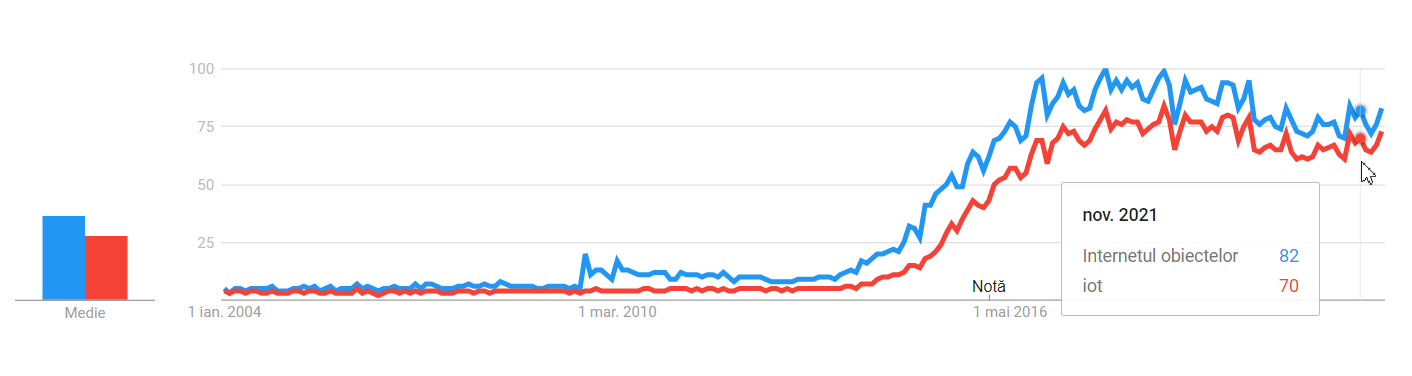
\includegraphics[width=\textwidth]{images/trends_iot.png}
\end{figure}


\section{Structura lucrării}

Capitolul curent a oferit o perspectivă de ansamblu asupra motivației, scopului și temei lucrării. În cele ce urmează, capitolul 2 va prezenta o serie de noțiuni fundamentale pentru înțelegerea subiectelor tratate, oferind definiții și explicații pentru diverse concepte întâlnite în domeniul \acrshort{iot} sau al testării sistemelor informatice. Va fi analizată apoi literatura relevantă temei în vederea conturării obiectivelor lucrării. Capitolul 3 conține o descriere atât teoretică, cât și tehnică a sistemelor \acrshort{iot}, oferind definiții riguroase și exemple de protocoale, arhitecturi și dispozitive utilizate în practică. În capitolul 4 găsim motivația pentru realizarea unui set de aplicații de evaluare pentru tehnicile de testare și descrierea implementării tehnice a unui astfel de \textit{benchmark}. Capitolul 5 continuă prin evaluarea câtorva tehnici de testare pe setul de aplicații propus anterior. Vor fi analizate o serie diversă de tehnici cum ar fi testarea funcțională și de integrare, testarea exploratorie folosind algoritmi de \textit{fuzzing}, analiză statică pentru descoperirea de vulnerabilități în codul sursă, iar în final câteva elemente de analiză cu modelare formală. Concluziile și subiectele ce rămân deschise pentru o cercetare viitoare vor fi expuse în capitolul 6. La finalul lucrării se vor regăsi glosarul termenilor și abrevierilor, bibliografia și anexele conținând cod sursă sau diagrame.
\chapter{Preliminarii}

În acest capitol vor fi prezentate noțiuni introductive despre natura sistemelor \acrfull{iot}, o prezentare sumară a caracteristicilor acestora și a contextului în care sunt utilizate, dar și noțiuni generale despre testare, tipurile de testare și câteva particularități pentru domeniul de interes. Vom continua prin analiza a câtorva studii cantitative sistematice despre testarea \acrshort{iot} pentru o mai bună întelegere a contextului, provocărilor și soluțiilor existente. În final, vom stabili obiectivele lucrării și cum vor fi acestea realizate.

\section{Noțiuni elementare}

\subsection{Despre IoT}

% Ce este IoT? Definitie si exemple relevante de sisteme

În analiza extensivă a literaturii \acrshort{iot} realizată de \cite{Nord2019} autorii au decis să utilizeze o definiție propusa de Ford Insights \cite{insight2017internet} (tradus din engleză):

% In this research, the Internet of Things (IoT)
% is defined as the interconnection of machines
% and devices through the internet, enabling
% the creation of data that can yield analytical
% insights and support new operations. For
% brevity and in keeping with current usage,
% Forbes refers to major technology categories
% such as IoT, artificial intelligence or robotics
% as technologies. It is recognized that each of
% the technology categories comprises multiple
% technologies and capabilities. For example,
% IoT is dependent upon sensors, wireless
% communications, networks, cloud, storage, etc.

\say{{[}...{]} \acrfull{iot} este definit ca interconectarea computerelor și dispozitivelor prin internet, dând posibilitatea de a genera date ce pot servi analizei și creerii de noi operațiuni. {[}...{]}}

Alte lucrări precum \cite{Lee2015} și \cite{Huang2015} preferă definiții mai largi, considerând că orice dispozitiv fizic conectat la internet este parte a \acrshort{iot}. Pentru o viziune mai clară, vom considera că \textbf{\acrshort{iot}} este reprezentat de totalitatea dispozitivelor și computerelor conectate la internet, care colectează sau procesează date, ori interacționează cu mediul înconjurător. Astfel, acest tip de sisteme au caracter \emph{heterogen}, pot fi \emph{distribuite} pe spații geografice întinse, utilizează tehnologii de comunicare \emph{wireless} și cresc rapid în complexitate o dată cu extinderea datorită \emph{interconectării} unui număr mare de părți.

% Ce sunt event-driven systems? Ce sunt sistemele heterogene?

% https://docplayer.net/15630715-Event-driven-applications-costs-benefits-and-design-approaches-gartner-application-integration-and-web-services-summit-2006.html
% https://www.redhat.com/en/topics/integration/what-is-event-driven-architecture

Un mod important de a privi sistemele \acrshort{iot} este să le vedem a fi \acrfull{edas}. Un \textbf{\acrshort{eda}} este un sistem construit în jurul producerii și consumului de \emph{evenimente}. Un eveniment reprezinta orice schimbare de stare a sistemului ca întreg. Acestea pot fi generate atât de senzori care monitorizează mediul, cât și de interacțiunea dintre om și computer sau simpla trecere a timpului. Transmiterea lor se poate face centralizat cu ajutorul unui distribuitor (\textit{message broker}) sau descentralizat în model \acrfull{p2p}. Consumatorii evenimentelor pot genera noi evenimente în urma procesării.

Definim informal un sistem \emph{heterogen} fiind un sistem în care părțile sale componente au în general natură diferită, concret în cazul pe care îl tratăm, heterogenitatea este dată de varietatea dispozitivelor \emph{hardware}, tehnologiilor \emph{software} și de interconectarea unui număr mare de astfel de componente în medii impredictibile. Astfel, putem trage concluzia că un sistem \acrshort{iot} este un \acrshort{eda} cu caracter heterogen în care software-ul este strâns legat de hardware spre deosebire de computerele de uz general. 

% Despre testare functionala si ne-functionala

\subsection{Despre testare}

% DONE: de scris despre SUT - system under test

\textbf{Testarea funcțională} a fost introdusă conceptual de \cite{Howden1980}, acesta propunând tratarea programelor ca o colecție integrată de funcții. Practicile și viziunile asupra metodelor de testare a aspectelor funcționale s-a rafinat continuu de-a lungul anilor, majoritatea eforturilor fiind îndreptate spre testarea software în medii izolate. În general, testarea funcțională presupune testarea comportamentului unui program în diferite scenarii ignorând detaliile de implementare, acesta fiind tratat ca un \textit{black box}. În contextul \acrshort{iot}, \cite{Corts2019} observă că majoritatea eforturilor de testare se duc spre aspectele funcționale, însă acestea reprezintă doar o singură piesă din multitudinea de de proprietăți ce asigură calitatea și buna funcționare a dispozitivelor.

În cazul testării aspectelor funcționale putem împărți testarea pe mai multe nivele, acestea fiind în general considerate: testarea unitară, adică testarea izolata a unei singure funcționalități, testarea de integrare, adică testarea funcționării corecte atunci când mai multe părți ale sistemului sunt implicate în realizarea unei funcționalități și în final testarea de sistem, care evident se referă la testarea întregului sistem, acesta putând să fie compus din mai multe componente \textit{software} și \textit{hardware}.

\textbf{Testarea aspectelor nefuncționale} se concentrează asupra unei game largi de probleme cum ar fi securitatea, conectivitatea, rezistența la stres și multe altele ce pot influența în mod indirect funcționarea unui sistem.

% Securitate, punct special

Un interes aparte în prezenta lucrare va fi acordat testării securității, deoarece este unul din subiectele de cel mai mare interes în rândul utlizatorilor și al producătorilor, așa cum constată \cite{Ahmed2019} și \cite{Lee2015}. Compromiterea securității \acrshort{iot} poate duce la nefuncționarea corectă, expunerea de date confidențiale sau chiar punerea în pericol de vieți omenești în cazul infrastructurilor critice.

% Relevanta in contextul IoT al notiunilor de mai sus

În contextul \acrshort{iot}, testarea prezintă particularități aparte, deoarece spre deosebire de testarea în arii clasice ale dezvoltarii \textit{software}, unde nivelul \textit{hardware} poate fi considerat sigur și suficient testat, aici avem de a face cu o legătură strânsă între \textit{software} și \textit{hardware}, ambele fiind insuficient testate și cu capabilități reduse.

% Dificultati in sistemele heterogene eda
% http://www.edwardcurry.org/publications/Hasan_DEBS_2012.pdf

\section{Analiza literaturii existente}

Pentru realizarea lucrării am parcurs articolele științifice din cardul conferințelor și jurnalelor recunoscute, dar și publicații private și independente din industrie. În continuare vom contura o imagine de ansamblu a metodologiilor, tehnicilor, practicilor și uneltelor utilizate pentru testarea sistemelor \acrshort{iot}. răspunzând la o serie de întrebări pe baza articolelor analizate: 

\begin{itemize}
    \item[] \textbf{Q1}. Care sunt aspectele sistemelor IoT pentru care există cel mai mare interes din punct de vedere al testării, atât pentru utilizatori cât și pentru producători?
    \item[] \textbf{Q2}. Care sunt metodologiile și uneltele de testare curente și cum acoperă acestea nevoile constatate anterior?
    \item[] \textbf{Q3}. Care sunt principalele obstacole întâmpinate de cercetători și dezvoltatori?
    \item[] \textbf{Q4}. Cum putem compara obiectiv diferite metodologii și eficiența acestora în a doborî obstacolele descoperite?
\end{itemize}

Motivația pentru \textbf{Q1} este nevoia de a afla care sunt ariile în care utilizatorii și producătorii își doresc o îmbunătățire a situației curente, astfel creăm posibilitatea de valoare adăugată pentru industrie cât și pentru mediul academic. \textbf{Q2} urmărește să stabilească starea curentă a tehnologiilor și metodologiilor, iar \textbf{Q3} să găsească principalele lipsuri ale stării curente, astfel ne putem îndrepta cercetarea spre nevoile concrete ale utilizatorilor, producătorilor și cercetătorilor. Răspunzând la \textbf{Q4} vom înțelege care sunt pașii necesari pentru a avansa în domeniul testării \acrshort{iot} și cum putem înlesnii acest proces și pentru alți cercetători. 

\subsection*{Q1. Care sunt aspectele sistemelor IoT pentru care există cel mai mare interes din punct de vedere al testării, atât pentru utilizatori cât și pentru producători?}

O analiză sistematică a 478 de articole publicate în perioada 2009 - 2017 realizată de \cite{Ahmed2019}, propune o taxonomie cuprinzătoare pentru cercetarea din domeniul \acrshort{iot}, clasele cele mai generale fiind: asigurarea calității (\textit{en. \acrlong{qa}}), performanța dispozitivelor, confidențialitate și încredere, securitate și testare. Efortul de cercetare este îndreptat cu precădere spre calitatea și securitatea sistemelor \acrshort{iot}, aspect tratat în 68 de lucrări. Arii similare cu un număr semnificativ de lucrări sunt \textit{design}-ul protocoalelor și arhitecturilor sigure cu 165 de lucrări și testarea securității cu 51 de lucrări. Privind aceste cifre, putem observa o atenție sporită oferită securității, aceasta fiind prezentă în multiple categorii. Consider justificat acest interes deoarece impactul digitalizării mediului înconjurător aduce toate riscurile asociate sistemelor informatice în viața cotidiană, dar și în infrastructuri critice. \cite{Lee2015} susțin această opinie, considerând că numărul în creștere al dispozitivelor interconectate poate crea reacții în lanț dezastroase în cazul unei breșe de securitate. Aceștia accentuează nevoia ca \textit{business}-urile să ofere interes sporit și să depună efort pentru asigurarea securității și confidențialității sistemelor produse.

Observăm ca securitatea este tema comună a multor lucrări, așa că o vom considera alături de funcționarea corectă a sistemelor, problema principală în IoT.

% DONE: mai trebuie sa scriu aici

\subsection*{Q2. Care sunt metodologiile de testare curente și cum acoperă acestea nevoile constatate anterior?}

Deși metodologiile de testare ale sistemelor \acrshort{iot} sunt variate și în număr mare, acestea nu au suport empiric foarte solid. Pentru metodele formale de analiză și testare cum ar fi \textit{model-based testing} (testarea bazată pe modelare formală) sau \textit{runtime verification} (verificarea în timpul execuției), \cite{Ahmed2019} constată că există un număr restrâns de experimente care să ateste eficiența și un număr și mai restrâns de inițiative de adoptare în industrie. Consider că una din posibilele cauze este dificultatea de a construi un set de proprietăți matematice suficient de cuprinzătoare pentru a aduce valoare suficientă, dar și efortul mare necesar pentru a implementa aceste metode de analiză. Alte metode formale de testare utilizează metode de analiză statistică a comportamentului dispozitivelor și sistemelor. 

Protocoalele de comunicație reprezintă un subiect de interes pentru testare. Avem de a face atât cu verificare formală, testare aleatoare sau testarea conformității cu specificațiile. Spre deosebire de dezvoltarea software generală unde protocoalele sunt considerate a fi testate exhaustiv deja, în dezvoltarea sistemelor \acrshort{iot} acestea încă reprezintă un teritoriu explorat insuficient. 

Interesați de testarea interoperabilității și integrării sistemelor, \cite{Bures2020} observă o serie de publicații care se concentrează pe testarea combinatorială, \textit{path-based testing}, dar și tehnici de testare individuală clasice care combinate pot reprezenta o soluție pentru testarea de integrare. 

\cite{Corts2019} constată că testarea de performanță, testarea funcțională și de utilizabilitate reprezintă cele mai întâlnite abordări din literatura evaluată, cu apariții în 27\%, respectiv 12\% și 14\% din articolele analizate. De asemenea, aceștia observă o ambiguitate în ceea ce privește utilizarea termenilor de "testare funcțională" și "testare de sistem" față de testarea software generală unde sunt utilizați cu mult mai multă precizie. Autorii atribuie această ambiguitate naturii heterogene și distribuite a sistemelor, propunând că noi tehnici trebuiesc explorate. 

În sfera practică a testării, \cite{Dias2018} realizează o listă a uneltelor software și platformelor utilizate în industrie. Întâlnim unelte orientate pe testarea individuală a dispozitivelor, respectiv a codului care se execută pe sistemele \textit{embeded}, dar și pentru testarea rețelelor. De asemenea, întâlnim soluții de testare pentru toate nivelele de la testare unitară la testare de acceptanță, însă niciuna nu oferă o acoperire integrală și nici universală, acestea fiind adesea legate de o platformă sau tehnologie anume. % TODO: de continuat cu cateva exemple concrete (nu-i urgent)

\subsection*{Q3. Care sunt principalele obstacole întâmpinate de cercetători și dezvoltatori?}

Un aspect semnalat de toate lucrările analizate este caracterul heterogen al sistemelor \acrshort{iot}, acestea fiind compuse din dispozitive și software produse de multiplii terți, o gamă largă de protocoale de comunicație și configurații posibile. \cite{Lee2015} expun provocările principale ale domeniului din perspectiva dezvoltatorilor, securitatea, confidențialitatea și haosul fiind principalele provocări. Prin haos, autorii se referă la plenitudinea de standarde, protocoale, comunicații complexe și dispozitive puțin testate ce sunt utilizate în practică în momentul de față. Acest caracter \textit{haotic} prezintă un risc crescut de a genera evenimente negative în infrastructuri critice cum ar fi cele medicale sau industriale. O altă perspectivă practică este prezentată de \cite{Dias2018}, care concluzionează că există o lipsă de unelte software destinate pentru testarea sistemelor heterogene și distribuite în mod automat, majoritatea soluțiilor fiind ancorate într-un set rigid de tehnologii sau manufacturieri. În plus, lipsesc soluții de testare pentru caractere nefuncționale ale sistemelor cum ar fi securitatea, confidențialitatea sau \textit{management}-ul actualizărilor software.

Atât \cite{Corts2019}, cât și \cite{Ahmed2019} semnalează necesitatea, dar și dificultatea creării de noi tehnici și metodologii pentru testarea sistemelor heterogene și distribuite, deoarece cele pentru sistemele tradiționale nu sunt eficiente sau aplicabile pentru industria \acrshort{iot}. Încă o provocare este reprezentată de compromisul dintre securitate și optimizarea costurilor de producție a dispozitivelor, \textit{hardware}-ul mai ieftin nu dispune de capabilități de securitate foarte avansate, producătorii fiind astfel puși în dificultate. Spre deosebire de sistemele clasice unde considerăm protocoalele și \textit{hardware}-ul suficient testate, în dezvoltarea produselor \acrshort{iot} aceste nivele nu sunt încă suficient acoperite.

\subsection*{Q4. Cum putem compara obiectiv diferite metodologii și eficiența acestora în a doborî obstacolele descoperite?}

Deși articolele analizate conțin o viziune cuprinzătoare asupra tehnicilor, metodologiilor și soluțiilor de testare, niciunul din acestea nu menționează metode de evaluare și comparare obiectivă. Luând în considerare lipsa de date empirice pentru validarea diferitelor metode de testare, lipsă constată de articolele în cauză, putem deduce că există o necesitate pentru stabilirea unui cadru de comparare și evaluare obiectivă pus la dispoziție cercetătorilor. Fără acest cadru, progresul spre doborârea provocărilor impuse de natura domeniului nu poate fi cuantificat cu ușurință. Acest lucru lasă loc interpretărilor și aprecierilor calitative subiective care au o contribuție minimală la cunoașterea științifică.

Observăm că și în alte arii există necesitatea metodelor obiective de evaluare și comparare, de exemplu în testarea aplicațiilor \textit{web} \cite{Garousi2013} constată că fiecare articol publicat utilizează un alt set de aplicații pentru evaluarea tehnicii de testare propuse, astfel compararea obiectivă a articolelor devine dificilă. Alt exemplu este reprezentat de \cite{Brockman2016} în sfera \textit{reinforcement learning}, autorii propunând un mediu unitar cu multiple probleme de reper (\textit{en. benchmark}) pentru evaluarea și compararea algoritmilor propuși de cercetători.

\section{Obiective}

În urma analizei făcute asupra literaturii existente, am identificat o serie de caracteristici definitorii pentru sistemele \acrlong{iot}, acestea sunt hetereogene, distribuite, prezintă interacțiuni complexe, produc și procesează cantități mari de date și sunt integrate în medii fizice. Toate acestea aduc o serie unică de provocări pentru dezvoltarea și testarea atât a \textit{software-}-ului, cât și a \textit{hardware}-ului. Aceste provocări sunt dificile și puțin explorate în comparație cu provocările din ariile clasice de dezvoltare \textit{software} precum dezvoltarea aplicațiilor web. 

Pentru a contribui la cunoștințele din domeniul testării sistemelor \acrshort{iot}, lucrarea de față își propune să realizeze următoarele obiective:

\begin{itemize}
    \item să stabilească un cadru teoretic și tehnologic pentru sistemele \acrshort{iot}, familiarizând cititorul cu caracteristicile, metodele de proiectare, dezvoltare și testare ale acestor sisteme, precum și obstacolele și provocările existente (în capitolul 3)
    
    \item să prezinte un set de aplicații \acrshort{iot} construit pentru a servi la compararea metodelor de testare și să argumenteze relevanța acestuia (în capitolul 4)

    \item să exemplifice utilizarea setului de aplicații pentru evaluarea diferitelor tehnici de testare întâlnite în literatură sau practică, să discute avantajele și dezavantajele lor și să constate eficiența lor (în capitolul 5)
\end{itemize}
\chapter{Modelarea sistemelor Internet of Things}

Pentru o analiză cât mai riguroasă este nevoie de o înțelegere profundă a sistemelor testate. În acest capitol vom oferi o imagine de ansamblu asupra rețelelor \acrshort{iot} ilustrând caracteristicile acestora cu exemple reale din diferite industrii. Pe baza exemplelor expuse vom discuta despre caracteristicile arhitecturale ale rețelelor, diferitele părți componente, topologiile comune și care este parcursul fluxurilor de date. Deoarece nu există o viziune unificată a modului în care ar trebui descrise arhitecturile acestor rețele particulare, vor fi expuse mai multe alternative și voi argumenta care este cea mai potrivită pentru a fi utilizată. 

Arhitecturile specifice \acrshort{iot} impun anumite constrângeri metodelor de comunicație, așa că vom explora care sunt cele mai comune protocoale de comunicație utilizate, care sunt particularitățile lor și care este motivația din spatele utilizării acestora. Nu ne vom rezuma doar la protocoalele dintr-un singur nivel al modelului \acrfull{osi}, ci vom urmări o privire de ansamblu, un interes special va fi acordat protocoalelor precum \textit{Zig-Bee} care este proiectat special pentru \acrshort{iot} și se întinde pe mai multe nivele \acrshort{osi}.

Canalele de comunicație au nevoie de părți comunicante, așa că vom continua prin a analiza dispozitivele și caracteristicile acestora utilizate în sistemele \acrshort{iot}, un punct important în această discuție fiind despre limitările hardware impuse de eficiența costurilor și cum acest aspect afectează capabilitățile de securitate. Deoarece software-ul este strâns legat de hardware în acest domeniu discuția va fi extinsă și asupra interacțiunii dintre cele două, în special despre modul în care dezvoltarea sau testarea uneia dintre componente o afectează pe cealaltă.

În finalul capitolului vom trece din planul tehnic și tehnologic în cel teoretic și vom modela formal și riguros rețelele \acrshort{iot} folosindu-ne de teoria grafurilor și teoria automatelor finite. Vor fi descrise atât topologiile și fluxurile de date fizice, cât și fluxurile la nivel logic. Ne propunem să obținem o viziune clară asupra proprietăților acestor sisteme pentru a putea exprima mai ușor aspectele testate și pentru a deschide calea spre metode de testare formală cum ar fi cele bazate pe \acrfull{smt}.

Un material suplimentar va fi reprezentat de un studiu de caz asupra sistemelor din locuințele inteligente unde vom identica aspectele discutate anterior și vom ilustra prin exemple aplicarea modelelor teoretice pentru descrierea unui astfel de sistem. Locuințele inteligente vor reprezenta exemplul principal în capitolele ce urmează atunci când vom aduce în prim plan tehnicile de testare.

\section{Arhitectură}

Așa cum ne spun \cite{Khodadadi2016}, componentele fundamentale și arhicunoscute ale sistemelor \acrshort{iot} sunt dispozitivele cu capabilități senzoriale, apelarea de servicii de la distanță, comunicarea peste rețea și procesarea de evenimente într-un context specific. Aceste părți componente puse împreună creează sisteme cu caracter puternic heterogen așa cum am menționat și anterior. Prin urmare, asigurarea interconectivității și interoperabilității devine un obiectiv greu de atins în lipsa unor procedee corespunzătoare de abstractizare. Aceste procedee de abstractizare se regăsesc în modelele arhitecturale propuse pentru sistemele \acrshort{iot}, modele pe care le vom analiza în paragrafele următoare, dar nu înainte de a arunca o scurtă privire asupra câtorva exemple practice.

Pentru a înțelege mai bine nevoia de abstractizare, să analizăm câteva exemple din lumea reală. Ne putem imagina o locuință inteligentă în care avem instalați senzori multiplii pentru temperatură, luminozitate, mișcare, etc. Aceștia transmit date către un computer central care le agregă și le pune la dispoziție utilizatorilor locuinței. De asemenea, utilizatorii își pot stabili pe baza datelor colectate o serie de automatizări, cum ar fi mișcarea draperiilor, reglarea temperaturii, încuierea ușii, etc. Toate facilitățile pot fi acționate de la distanță prin intermediul internetului. În plus, locuința este conectată la sistemul inteligent al municipalității pentru a comunica informații despre consumul de energie, apă sau alte resurse. În cadrul sistemului municipal, scenariul se repetă. Regăsim o serie de senzori, centre de comandă și dispozitive de acțiune. Este evident cât de rapid crește complexitatea chiar și într-un caz relativ restrâns.

Un alt exemplu poate fi reprezentat de o linie de producție industrială complet automatizată. Multiplii senzori colectează date despre funcționarea aparaturii. Unul sau mai multe centre de comandă interpretează datele pentru a orchestra brațele robotice din cadrul liniei de producție. Angajații respectivei fabrici pot interacționa cu sistemele acesteia pentru monitorizare și control manual atunci când este nevoie. Toate datele conectate sunt trimise către \textit{cloud}-ul companiei pentru analiza și optimizarea proceselor de producție. Acest gen de sisteme reprezintă o nișă specifică, anume \acrfull{iiot}. 

% TODO: sa bag niste diagrame misto cu un sistem smart home si cu unul industrial, poate chiar o diagrama din Node-RED

Modelele arhitecturale au evoluat în timp și continuă să evolueze, așa că le vom analiza în ordinea complexității lor.

\subsection*{\textit{3-layer}}
% TODO diagram 3 layer

\cite{MiaoWu2010} spune că în ciuda lipsei unei definiții unificate pentru \acrshort{iot}, arhitectura \textit{3-layer} este larg acceptată și cunoscută. Acest fapt este bine fundamentat, deoarece găsim referințe la acest model arhitectural în multiple publicații la care ne vom referi în paragrafele următoare. Nivelele componente ale acestei arhitecturi sunt:

\begin{enumerate}
    \item Nivelul de percepție (\textit{perception layer})
    \item Nivelul rețelei (\textit{network layer})
    \item Nivelul aplicației (\textit{application layer})
\end{enumerate}

Nivelul de percepție conține senzori, cititoare de \acrshort{rfid} sau coduri de bare, sisteme \acrfull{gps} sau camere de filmat. Acesta facilitează colectarea de date despre mediul înconjurător sistemului \acrshort{iot}. Identificăm cu ușurință acest nivel în exemplul nostru anterior, senzorii termici sau de mișcare, cât și dispozitivele de măsurat consumul de energie sau apă fac parte din acesta. Acest nivel poate fi de asemenea considerat a fi colecția de \textit{things} din \acrshort{iot}.

La nivelul rețelei întâlnim infrastructura care pune la dispoziție comunicarea dintre \textit{things}. Această infrastructură este formată din \textit{router}-e, \textit{switch}-uri, centre de procesare și management, etc. De exemplu, într-o locuință inteligentă rețeaua \textit{wireless} și centrul de control reprezintă nivelul de rețea.

Procesarea datelor și executarea fluxurilor specifice se petrece la nivelul aplicației. Acest nivel reprezintă totalitatea componentelor software și hardware care facilitează serviciile dorite de utilizator. De exemplu, software-ul de automatizare prezent pe centrul de comandă dintr-o locuință inteligentă face parte din acest nivel.

\cite{Lin2017} constată ca deși această arhitectură este fundamentală și simplă, funcționalitățile și operațiunile desfașurate de sistem la nivelul rețelei și aplicației sunt diverse și complexe. În opinia autorilor este nevoie de dezvoltarea unui nivel de serviciu \textit{service layer} care să medieze interacțiunea dintre rețea și aplicație. Acest nivel adițional ar facilita o mai mare flexibilitate sistemului.

\subsection*{\textit{5-layer}}
% TODO diagrama 5 layer

Arhitectura \textit{3-layer} nu conține metode de management suficient de bune și nu ia în considerare nevoia de a modela domeniile de \textit{business} în perspectiva \cite{MiaoWu2010}. Pentru a combate aceste dificultăți, autorii propun o arhitectura cu cinci nivele, după cum urmează:

\begin{enumerate}
    \item Nivelul de percepție (\textit{perception layer})
    \item Nivelul de transport (\textit{transport layer})
    \item Nivelul de procesare (\textit{processing layer})
    \item Nivelul aplicației (\textit{application layer})
    \item Nivelul \textit{business} (\textit{business layer})
\end{enumerate}

Primele două nivele corespund cu cele din arhitectura \textit{3-layer}, îndeplinind aceleași funcții. În continuare, nivelul de procesare preia o parte din atribuțiile nivelului aplicației din arhitectura anterioară. Din acest nivel fac parte bazele de date, \textit{cloud}-ul și toate celelalte aparaturi de procesare de date pentru a facilita utilizarea acestora la nivelul aplicației. În viziunea autorilor, această separare dintre procesare și utilizare în scopuri aplicate este necesară pentru flexibilitatea și scalabilitatea \acrshort{iot}.

În final avem de a face cu nivelul de \textit{business} care ar trebui să reprezinte un nivel de management peste nivelul aplicației, fiind preocupat de modelul de \textit{business} și dezvoltarea pe termen lung. Din păcate, autorii nu pun la dispoziție o descriere detaliată, aplicarea acestui tip de arhitectură rămânând la latitudinea dezvoltatorului. O imagine mai clară asupra nivelului de \textit{business} ne-o oferă \cite{Khan2012} specificând că acesta conține modelele de \textit{business}, grafice și organigrame bazate pe datele obținute din nivelul de aplicație. Scopul acestui nivel este să producă strategii și decizii de \textit{business}, deci este un nivel de interacțiune între om și mașină.

\subsection*{\textit{Service Oriented Architecture}}
% TODO: diagramă

O arhitectură orientată pe servicii, în orginal \acrfull{soa}, propune împărțirea componentelor și funcționalităților unui sistem un unități mici și independente numite servicii. Această arhitectură nu impune un număr fix de nivele, însă trebuie sa existe cel puțin un nivel care facilitează două activități fundamentale: descoperirea serviciilor (\textit{service discovery}) și invocarea acestora (\textit{service calling}). 

\cite{Khodadadi2016} susțin că acest tip de arhitectură asigură interoperabilitatea dispozitivelor heterogene, această proprietate fiind esențială pentru sistemele \acrshort{iot}. De asemenea, oferă și un exemplu de \acrshort{soa} adăugând un nivel de servicii în clasica arhitectură \textit{3-layer}. Funcționarea independentă a serviciilor asigură că sistemul va continua să funcționeze majoritar corect, chiar dacă un număr mic de servicii au încetat să funcționeze. Acest aspect este foarte important pentru fiabilitatea sistemelor, o proprietate de mare interes. Același tip de arhitectură este descris și de \cite{Lin2017} într-un meta-studiu.

O altă perspectivă asupra unui posibil tip de \acrshort{soa} vine din partea \cite{LuTan2010} care propune o arhitectură \textit{5-layer} modificată. Pe langă nivelul rețelei, aceștia introduc un nivel de coordonare al serviciilor care are rolul de a unifica comunicarea asigurând interoperabilitatea. Din păcate, nu sunt oferite detalii suplimentare despre implementarea acestui tip de arhitectură.

\subsection*{\textit{API-oriented}}

Deoarece arhitecturile de tip \acrshort{soa} sunt complexe, iar procesele de coordonare și descoperire a serviciilor necesită un efort considerabil de dezvoltare, alternative mai simple au fost introduse. \cite{Khodadadi2016} prezintă o imagine de ansamblu a arhitecturilor orientate spre \acrfull{api}. % TODO: sa continui aici, nu mai am idei

\section{Protocoale de comunicație}

În discuția anterioară despre arhitectura sistemelor \acrshort{iot} am observat că un rol important este jucat de mecanismele de comunicare. Aceste sisteme sunt nevoite să coordoneze un număr mare de dispozitive și să transmită o cantități enorme de date într-un mod fiabil, rapid și rezistent la șoc. De aceea sunt utilizate o gamă largă de protocoale de comunicație, fiecare cu avantajele și dezavantajele sale, în încercarea de a depăși provocările impuse de natura distribuită și heterogenă a sistemelor. 

Este necesar să fim familiari cu modelul \acrfull{osi} pentru o bună înțelegere a diferențelor dintre diferitele protocoalele utilizate. Deoarece \acrshort{iot} este un domeniu volatil în care hardware-ul este în strânsă legătură cu software-ul, 


TODO: de vorbit despre protocoalele specifice

TODO: de inclus rezumatul despre Event-Driven-Systems

\section{Caracteristicile dispozitivelor}

\section{Model teoretic}

În încercarea de a crea un cadru obiectiv pentru analiza sistemelor IoT din punct de vedere al proprietăților și potențialelor defecte din acestea, vom introduce câteva noțiuni teoretice pentru descrierea acestor sisteme. În secțiunea anterioară am discutat despre comunicarea fizică a dispozitivelor, diferitele topologii pe care le-am putea întâlni și protocoalele utilizate. Vom extinde discuția spre fluxurile logice prezente în aceste rețele, deoarece deși topologiile de tip stea sunt des întâlnite, nodul central servește ca un intermediar pentru fluxuri logice între un număr mare de dispozitive, acestea neputând fi reduse la o interacțiune nod central - dispozitiv.

Vom folosi ca fundație specificația propusă de \cite{Paduraru2021}, deoarece propune o descriere formală a rețelelor IoT folosind teoria grafurilor pentru a ușura automatizarea proceselor de testare, fără a fi nevoie să se specifice detalii tehnice precum protocoalele sau software-ul utilizat. Autorii propun să vizualizăm o aplicație IoT ca o serie de perechi \textit{input}-\textit{output} care pot fi descrise de un graf orientat G în modul următor:

\begin{enumerate}
    \item orice vârf $v \in V$ reprezintă un dispozitiv fizic pe care se execută unul sau mai multe procese software
    \item o muchie orientată $e \in E$ de la un vârf $v_1$ la un vârf $v_2$ descrie un flux de date de la \textit{output}-ul lui $v_1$ spre \textit{input-ul} lui $v_2$
    \item orice vârf $v \in V$ este consumatorul datelor pentru un set de producători $V_{in}(v) = \Big{\{} v_{in} \; \Big{|} \; \exists v \in V \land (v_{in}, v) \in E \Big{\}}$
    \item orice vârf $v \in V$ este producător pentru un set de consumatori $V_{out}(v) = \Big{\{} v_{out} \; \Big{|} \; \exists v \in V \land (v, v_{out}) \in E \Big{\}}$
    \item orice vârf $v \in V$ este caracterizat de un \textit{buffer} de \textit{input} și unul de \textit{output}, aceștia fiind descriși de relația producător consumator astfel încât: $Buffer_{in}(v) = \bigcup_{v_{in} \in V_{in}(v)} Buffer_{out}(v_{in})$ și analog $Buffer_{out}(v) = \bigcup_{v_{out} \in V_{out}(v)} Buffer_{in}(v_{out})$
    \item graful $G$ este dinamic, vârfuri și muchii putând fii adăugate sau eliminate în timpul funcționării rețelei
\end{enumerate}

% TODO: de adaugat o diagrama si de explicat pe ea

Un aspect important discutat de autori este că muchiile rețelei trebuiesc privite dintr-o perspectivă probabilistă, anume ele pot lipsi în timpul funcționării sistemului. De exemplu, un senzor ar putea fi deconectat, fără energie sau să comunice date la intervale foarte lungi de timp. O viziune mai clară asupra acestui aspect o putem avea privind Figura ... Observăm că unele muchii sau vârfuri din graf sunt obligatorii pentru funcționarea sistemului, eliminarea lor făcând imposibilă o execuție coerentă. Acest set de vârfuri și muchii obligatorii sunt notate $V_r$ și $E_r$ și determină graful funcțional minimal $G_r$. % TODO de adaugat figura si de explica

Dacă considerăm orice graf $G \in G_{total}$ o stare posibilă a rețelei (ie. $G$ conține toate muchiile și vârfurile obligatorii), observăm ca avem de a face cu un automat finit. Putem descrie stările acestui automat considerând $S = \Big{\{} G  \; \Big{|} \; G \in G_{total} \land G_{r} \subseteq G \Big{\}}$ și operațiile posibile de modificare ale grafului $\Sigma = \Big{\{} \text{adăugare muchie}, \text{ștergere muchie}, \text{ștergere vârf}, \text{adăugare vârf} \Big{\}}$.

% TODO poate ar trebui sa citesc lucrurile astea de undeva?
% TODO poate ar fi interesant totusi sa extind un pic ideea? ar fi interesant pentru fuzzing

O descriere mult mai precisă a sistemului ar putea fi reprezentată de utilizarea lanțurilor Markov deoarece muchiile opționale au probabilități asociate, însă această abordare depășește scopul lucrării de față.

Descrierea propusă de \cite{Paduraru2021} se concentrează pe fluxurile fizice de date dintre dispozitive, însă un aspect important al acestor tipuri de sisteme este reprezentat de fluxurile logice de date, așa cum am văzut în discuția anterioară despre arhitecturi și protocoale, datele colectate de un senzor sau generate de un utilizator pot influența multiple părți ale sistemului, de la simplii actuatori până la sisteme complexe de analiză și decizie.

% TODO: sa vad cum as putea vorbi despre flow-uri logice

Într-o manieră similară celei de mai sus putem descrie graful $G'$

% TODO: de citat paper-ul lui Stefanescu + Paduraru despre privitul ca graf
% TODO: de vazut cum s-ar putea descrie state-ul retelei cu teorie de la automatele finite
% TODO: de vorbit despre numarul imens de stari, caracterul continuu al masuratorilor, etc
% TODO: de subliniat distinctia dinstre comunicarea logica (la nivel de flow) si comunicarea fizica (la nivel de protocol/device) si de modelat comunicarea logica

\section{Studiu de caz: locuințe inteligente}

TODO: de inclus rezumatul despre smart home thread modeling

TODO: de inclus studiul de la trendmicro
\chapter{Construirea unei suite de aplicații pentru evaluarea 
tehnicilor de testare}

După cum am argumentat în capitolele precedente, sistemele \acrshort{iot} sunt complexe, heterogene și distribuite, caracteristici care aduc o serie de dificultăți greu de depășit în testare. Am oferit o argumentare detaliată asupra acestor aspecte în secțiunea \textbf{2.2.Q3}. Pentru a avansa în ce privește starea curentă a tehnicilor de testare avem nevoie de metrici cât mai obiective, care ar ușura munca cercetătorilor de a reproduce rezultate și de a le compara. În urma analizei literaturii din secțiunea \textbf{2.2.Q4}, am constatat imposibilitatea stabilirii unor astfel de metrici, deoarece majoritatea publicațiilor utilizează o suită proprie de aplicații pentru desfășurarea experimentelor. Astfel, a compara numărul de defecte descoperite, timpul sau alți parametri este irelevant, deoarece mediul variază. 

Regăsim aceeași concluzie enunțată de \cite{Paduraru2021}, în articolul lor care propune o specificație formală pentru descrierea sistemelor \acrshort{iot}. Pentru evaluarea riguroasă a specificației propuse este nevoie de construirea unei suite de aplicații cât mai apropiate de realitate. Această inițiativă este materializată și prezentată de lucrarea lui \cite{Cristea2022}. Aceasta va fi prezentată în paginile ce urmează evidențiind contribuțiile proprii, fără a omite perspectiva generală. 

Un aspect important al suitei de aplicații construit este faptul că este \textit{open-source}. Într-o industrie în care majoritatea producătorilor nu pun la dispoziție decât sursele deja compilate ale \textit{firmware}-ului, iar în multe cazuri acestea se află pe dispozitive ce nu permit accesarea lui, existența \textit{software}-ului \textit{open-source} este crucială pentru a crea un mediu transparent de experimentare. 

O observație importantă este că suita de aplicații este realizat în mare măsură imitând aplicațiile reale dintr-o locuință inteligentă, deoarece este unul din cele mai întâlnite scenarii de utilizare a tehnologiilor \acrshort{iot} și pentru că oferă un grad de complexitate și interconectare suficient de mic încât să fie realizat fără eforturi majore, dar și suficient de mare încât să mimeze comportamentul unui sistem real, aducând același tip de provocări.

În prezentul capitol, vom discuta despre modul de construire al suitei de aplicații și particularitățile fiecărei aplicații în parte, prezentând funcționalitatea și tehnologiile utilizate pentru realizarea ei. Ne vom concentra apoi asupra infrastructurii de interconectare a aplicațiilor și vom discuta despre protocoalele utilizate și motivația alegerii lor. Pentru a ilustra o situație cât mai apropiată de realitate aplicațiile sunt angrenate în fluxuri de automatizări orchestrate de o unitate centrală, analiza acestor fluxuri fiind de asemenea prezentă în acest capitol. După înțelegerea structurală a setului de aplicații vom vedeam cum îl putem folosi pentru compararea și analizarea tehnicilor de testare și cum poate fi acesta util pentru cercetători sau profesioniști. În final ne vom concentra asupra limitărilor și posibilelor îmbunătățiri ce ar putea fi aduse în viitor setului de aplicații.

\section{Descrierea aplicațiilor}

Pentru a ilustra cât mai bine o situație reală, aplicațiile utilizate au surse multiple, o parte fiind dezvoltate de echipe independente de studenți, o altă parte au fost scrise de echipa de cercetare \acrshort{sasha}, iar altele au fost obținute din surse publice. Au fost aduse modificări pentru a facilita integrarea, dar și pentru a introduce defecte (\textit{en. bugs}) artificiale pe lângă cele deja existente. Această diversitate se regăsește și în sectorul comercial, acolo unde dispozitive și software de la producători multipli sunt utilizate în medii complexe și condiții impredictibile. Considerăm că această abordare de construire a aplicațiilor este suficient de robustă și suficient de apropiată de realitate.

În paragrafele următoare vom analiza caracteristicile fiecărei aplicații \footnote{Codul sursă al aplicațiilor, infrastructura și documentația acestora pot fi găsite la \url{https://github.com/unibuc-cs/IoT-application-set}}, caracteristici precum modul de funcționare, tehnologiile utilizate pentru dezvoltare, dependența și interacțiunea față de alte aplicații sau relevanța pentru evaluarea tehnicilor de testare. Toate aplicațiile simulează procese des întâlnite în locuințele inteligente.

% ===================================================================== DONE
\subsection*{FlowerPower}

\textbf{Descriere}:  Un \textit{ghiveci inteligent} care expune prin intermediului unui \acrshort{api} supravegherea și îngrijirea plantelor. De asemenea poate notifica utilizatorul în legătură cu anumite schimbări legate de starea plantelor.

\textbf{Tehnologii utilizate}: \textit{C++} și \textit{GNU Makefiles} pentru dezvoltare, împreună cu bibliotecile \textit{Pistache} pentru servirea de cereri \acrfull{http}, \textit{RapidJson} pentru lucrul cu date în format \acrfull{json} și \textit{Mosquitto} pentru comunicarea cu un distribuitor de mesaje prin protocolul \acrfull{mqtt}. 

\textbf{În context}: Interacționează cu aplicația WindWow în legătură cu aspecte precum temperatura sau luminozitatea.

\textbf{Sursă}: Echipă de Studenți înscriși la cursul de Ingineria Programării, anul 2020.
% =====================================================================

% =====================================================================
\subsection*{WindWow}

\textbf{Descriere}:  O fereastră inteligentă ce permite monitorizarea temperaturii și luminozității din cameră, luminozitatea fiind reglabilă prin intermediul draperiilor acționate de utilizator de la distanță.

\textbf{Tehnologii utilizate}: \textit{C++} și \textit{CMake} pentru dezvoltare, împreună cu bibliotecile \textit{Pistache}, \textit{NLohmann-JSON} pentru lucrul cu date în format \acrshort{json} și \textit{Mosquitto}.

\textbf{În context}: Senzorii de luminozitate și temperatură colectează date relevante pentru o multitudine de alte dispozitive din rețea cum ar fi SmartFlower și SmartTV, care își pot calibra funcționarea în funcție de datele primite.

\textbf{Sursă}: Echipă de Studenți înscriși la cursul de Ingineria Programării, anul 2020.
% =====================================================================

% =====================================================================
\subsection*{Smarteeth}

\textbf{Descriere}: 

\textbf{Tehnologii utilizate}: 

\textbf{În context}: 

\textbf{Sursă}: Echipă de Studenți înscriși la cursul de Ingineria Programării, anul 2020.
% =====================================================================

% =====================================================================
\subsection*{SmartKettle}

\textbf{Descriere}:  

\textbf{Tehnologii utilizate}: 

\textbf{În context}: 

\textbf{Sursă}: Echipă de Studenți înscriși la cursul de Ingineria Programării, anul 2020.
% =====================================================================

% =====================================================================
\subsection*{SmartTV}

\textbf{Descriere}: 

\textbf{Tehnologii utilizate}: 

\textbf{În context}: 

\textbf{Sursă}: Echipă de Studenți înscriși la cursul de Ingineria Programării, anul 2020.
% =====================================================================

% =====================================================================
\subsection*{SmartOven}

\textbf{Descriere}: 

\textbf{Tehnologii utilizate}: 

\textbf{În context}: 

\textbf{Sursă}: Echipă de Studenți înscriși la cursul de Ingineria Programării, anul 2021.
% =====================================================================

% =====================================================================
\subsection*{SeraSmart}

\textbf{Descriere}: 

\textbf{Tehnologii utilizate}: 

\textbf{În context}: 

\textbf{Sursă}: Echipă de Studenți înscriși la cursul de Ingineria Programării, anul 2021.
% =====================================================================

% =====================================================================
\subsection*{SoundSystem}

\textbf{Descriere}: 

\textbf{Tehnologii utilizate}: 

\textbf{În context}: 

\textbf{Sursă}: Autorul prezentei lucrări
% =====================================================================

% TODO: de adaugat diagrame pentru astea doua de jos

% =====================================================================
\subsection*{PhilipsHue Simulator}

\textbf{Descriere}: 

\textbf{Tehnologii utilizate}: 

\textbf{În context}: 

\textbf{Sursă}: Autorul prezentei lucrări
% =====================================================================

% =====================================================================
\subsection*{Smart Vacuum Cleaner}

\textbf{Descriere}: 

\textbf{Tehnologii utilizate}:

\textbf{În context}: 

\textbf{Sursă}: Autorul prezentei lucrări
% =====================================================================

Observăm ca aplicațiile prezentate sunt variate atât din punct de vedere al tehnologiilor utilizate (\textit{C++}, \textit{Python}, \textit{Go}, \textit{Rust}), cât și din punct de vedere al funcționării lor, acestea acoperind o gamă largă de utilizări posibile în cadrul unei locuințe inteligente. 

% TODO: sa vorbesc un pic mai mult de tehnolgii si relevanta lor pentru iot
% TODO: sa vorbesc despre fluxurile de automatizari si sa descriu cateva

În secțiunea următoare vom prezenta modul în care aceste aplicații au fost integrate într-o suită coerentă cu fluxuri de intercomunicare complexe.

\section{Infrastructura}

Așa cum am menționat anterior, dispozitivele dintr-un sistem \acrshort{iot} sunt interconectate și fac parte din fluxuri de complexități variate. Pentru a ne păstra cât mai aproape de un sistem real, aplicațiile mai sus menționate au fost puse într-o rețea comună și orchestrate folosind o aplicație centrală, în general cunoscută sub numele de \textit{hub}. Rețeaua poate fi desfășurată (en. \textit{deployed} - \textit{deployment}) atât într-un mediu virtualizat folosind tehnologiile \textit{Docker} și \textit{docker-compose}, dar și într-un mediu cu hardware fizic folosind o serie de \textit{script}-uri de automatizare, dar și câteva operații manuale. În experimentele desfășurate am folosit atât mediul virtualizat, cât și un \textit{deployment} pe arhitectura \textit{x86} \footnote{TODO: } și pe \textit{ARMv7l} \footnote{TODO: ...} folosind un \textit{Raspberry Pi 2 Model B} \footnote{TODO: ...}. 

Punctul central al rețelei este reprezentat de aplicația \textit{hub}. Aceasta este responsabilă cu monitorizarea și orchestrarea tuturor dispozitivelor din rețea și permite implementarea fluxurilor de automatizare. \textit{Hub}-ul este o aplicație proprie dezvoltată folosind limbajul \textit{Python} și permite integrarea a două protocoale de comunicație în momentul de față: \acrshort{http} și \acrshort{mqtt}. Am ales să nu folosim o aplicație \textit{hub} comercială cum ar fi \textit{OpenHAB} sau \textit{Home Assistant}, deoarece avantajele aduse de o soluție personalizată din punct de vedere al timpului de integrare și al simplității au fost superioare.

Pentru a asigura omogenitatea comunicării într-un sistem cu componente heterogene, toate aplicațiile au specificații \textit{OpenAPI} \footnote{TODO: descrie openapi} pentru descrierea rutelor \acrshort{http} expuse și specificații \textit{AsyncAPI} \footnote{TODO: ...} pentru descrierea formatului mesajelor transmise prin intermediul protocolului \acrshort{mqtt}. Folosind \textit{OpenAPI Generator} \footnote{TODO: ...}, specificațiile \textit{OpenAPI} pot fi transformate în cod de interacțiune cu aplicațiile. Codul generat a fost utilizat în aplicația de hub pentru a oferi acces uniform la aplicații.

% TODO: de adaugat un listing cu openapi si asyncapi ca sa vedem cum arata

Față de protocolul \acrshort{http}, protocolul \acrshort{mqtt} operează în manieră \textit{publisher}/\textit{subscribe}, nu \textit{request}/\textit{reqsponse}, astfel devine necesară existența unui distribuitor de mesaje în rețea. Pentru această sarcină am utilizat \textit{Eclipse Mosquitto}, deoarece este un produs \textit{open-source} ușor de instalat și folosit atât în mediu virtualizat cât și nevirtualizat.

Întreaga configurație este stocată în câteva fișiere în format \acrfull{yaml} sau \acrshort{json}, aceasta specificând numele și calea aplicațiilor, porturile de rețea expuse și alți parametrii specifici. De asemenea conține informații despre aplicația \textit{hub} și serviciile externe necesare (cum ar fi distribuitorul de mesaje). Configurația este citită de utilitarele construite pentru a facilita cele mai comune operații: compilarea aplicațiilor, rularea aplicațiilor pe mediul local virtualizat sau nu, executarea unor teste, repornirea sau oprirea aplicațiilor, instalarea dependințelor software, etc.

% TODO: diagrama retea, aplicatii, hub, etc

% TODO: diagrama docker

\textit{Docker} este o soluție software pentru izolarea aplicațiilor în containere. Față de mașinile virtuale clasice care fie utilizează facilitățile de virtualizare ale unității centrale de procesare, fie emulează în întregime o unitate centrală, \textit{Docker} pune la dispoziție un strat de abstractizare între aplicații și sistemul de operare astfel încât acestea se execută într-un mediu izolat denumit container, fără acces la restul sistemului. De asemenea, configurarea dependințelor și mediului din container în care va fi executată aplicația sunt specificate în mod textual, în asa numetele \textit{Dockerfiles}. Această abordare aduce o serie de avantaje printre care se numără o mai bună securitate pentru un cost mic de performanță și o bună reproductibilitate a mediilor. Pentru a orchestra mai multe containere folosim \textit{docker-compose} care poate fi configurat de asemenea în mod textual. Acesta permite și configurarea de topologii, medii de stocare și interacțiunea cu sistemul gazdă.

Utilizarea suitei de aplicații folosind \textit{Docker} este convenientă, deoarece consumă puține resurse și nu necesită pregătiri suplimentare, însă pentru a simula un scenariu mai apropiat de realitate, aplicațiile pot fi de asemenea puse pe dispozitive hardware fizice cum ar fi \textit{Raspberry Pi}. Am pus la dispoziție scripturile necesare pentru compilarea aplicațiilor și instalarea dependințelor pentru un sistem \textit{Raspbian ARMv7l}. Aplicațiile împreună cu \textit{hub}-ul și distribuitorul de mesaje au fost desfășurate pe mai multe \textit{Raspberry Pi's} conectate prin \textit{wi-fi}.

% TODO: diagrama raspberry pi

\section{Extinderea suitei de aplicații}

Deoarece există un număr foarte mare de posibile tipuri de sisteme \acrshort{iot} și utilizări ale acestora, suita de aplicații nu acoperă decât un mic număr din total. Astfel, încurajăm extinderea și îmbogățirea suitei cu aplicații și fluxuri de automatizare proprii atât din partea cercetătorilor cât și a profesioniștilor. Pașii pentru includerea unei noi aplicații sunt simplii și puțini la număr, astfel asigurând un proces cât mai puțin anevoios. În rândurile ce urmează vom parcurge ce caracteristici trebuie sa aibă o nouă aplicație și ce pași trebuie urmați pentru includerea ei.

\textbf{Caracteristici necesare}:
\begin{enumerate}
    \item Aplicația trebuie sa comunice folosind cel puțin unul din protocoalele \acrshort{http} sau \acrshort{mqtt}.
    \item Sunt necesare specificații \textit{OpenAPI} și/sau \textit{AsyncAPI} în funcție de protocoalele folosite.
    \item Codul trebuie sa poată fi compilat pentru arhitectura \textit{x86} sau să poată fi cel puțin executat într-un emulator
\end{enumerate}

\textbf{Integrarea în suită} \footnote{Tutorialul complet poate fi găsit la adresa \url{https://github.com/unibuc-cs/IoT-application-set/blob/master/HOW_TO_ADD_AN_APP.md}}:
\begin{enumerate}
    \item Crearea configurațiilor necesare pentru generarea de clienți de comunicare (momentan doar pentru \acrshort{http}).
    \item Punerea la dispoziție a unui \textit{script} de instalare al dependințelor aplicației.
    \item Punerea la dispoziție a unui \textit{script} de compilare a aplicației pentru arhitecturile țintă.
    \item Punerea la dispoziție a unui \textit{script} pentru executarea aplicației pe un port de rețea arbitrar.
    \item Crearea unei configurații în format \textit{Dockerfile} și adăugarea unei intrări în configurația generală a suitei.
    \item Copierea codului sursă a noii aplicației în directorul corespunzător.
\end{enumerate}

Deși recomandăm integrarea aplicațiilor \textit{open-source}, în cazul în care sursa nu este disponibilă, se pot omite pașii de compilare și copiere ale sursei aplicației. Este necesar însă să ne asigurăm ca binarele puse la dispoziție pot fi executate pe arhitectura \textit{x86} fie direct, fie prin intermediul unui emulator.

\section{Defecte, evaluare și limitări}

Scopul suitei de aplicații este compararea metodelor de testare, așa cum am menționat anterior. Pentru a oferi un reper relevant, este necesar ca aplicațiile să conțină defecte realiste. Cum aceste aplicații au fost dezvoltate de multiple echipe de de studenți, conțin în mod natural o serie de defecte, defecte pe care le-am identificat în urma testării funcționale a suitei, dar despre acest proces vom discuta în capitolul următor. Pe lângă defectele existente, am considerat necesară îmbogățirea suitei cu o gamă mai largă de defecte. Acestea au fost introduse în codul aplicațiilor sau în regulile de automatizare din aplicația \textit{hub}, unele defecte fiind o combinație din ambele.

Deoarece una din caracteristicile principale ale \acrshort{iot} este numărul mare de părți comunicante, am ales să împărțim defectele descoperite și injectate în trei categorii bazate pe nivelul de interacțiune dintre părțile sistemului. Aceste categorii sunt următoarele:

\begin{enumerate}
    \item Defecte la nivel de aplicație - acestea afectează doar aplicații individuale, efectele comune fiind funcționarea incorectă sau oprirea funcționării în totalitate
    \item Defecte la nivel de flux de automatizare - caracterizate de rezultatul incorect la finalul executării unui singur flux de automatizare ce conține multiple aplicații
    \item Defecte la nivel de persistență în sistem - atunci când execuția a mai multe fluxuri de automatizare care nu sunt disjuncte duce la funcționarea incorectă a întregului sistem
\end{enumerate}

În general, defectele din prima categorie au fost cel mai des abordate în literatură, majoritatea soluțiilor existente concentrându-se pe acestea. Pe de altă parte, defectele din celelalte categorii au un grad de dificultate în detectare mult mai ridicat, deoarece sunt cauzate în general din motive de concurență și sunt în strânsă legătură cu domeniul specific în care este utilizată aplicația. Să luam un exemplu pentru a ne face o imagine mai clară, un defect din categoria întâi poate fi reprezentat de un acces invalid de memorie care cauzează un răspuns întârziat, un răspuns cu date aleatorii sau chiar nefuncționarea completă a aplicației. Metricile de detectare sunt clare și independente de logica concretă a aplicației. Un defect din categoria a treia este mult mai subtil și mai complex, spre exemplu să considerăm ca un senzor de lumină inteligent comandă acționarea draperiilor în funcție de nivelul de luminozitate înregistrat. Utilizatorul comandă manual draperiile în timp ce acestea sunt în curs de acționare și cauzează blocarea mecanismului. În acest caz, detectarea defectului nu mai este la fel de evidentă, iar producerea acestuia necesită alinierea mai multor evenimente independente. 

În studiul realizat de \cite{Zhou2021} se menționează o clasă de defecte cauzate de acțiuni impredictibile în cadrul fluxurilor de automatizări. Această clasă de defecte este ceea ce noi considerăm a fi defectele de nivel doi și trei în categorisirea proprie. Conform autorilor studiului, cauzele acestei clase de defecte sunt următoarele:

% TODO: cum zic race condition in romana?
\begin{enumerate}
    \item \textit{race condition} între diferite fluxuri
    \item evenimente lipsă sau procesate într-o ordine imprevizibilă
    \item acțiuni duplicate sau în conflict
\end{enumerate}

% TODO: de vorbit despre nivelele de buguri

În rândurile de mai jos vom analiza câteva exemple de defecte existente și introduse din toate cele trei categorii numite \footnote{O listă completă a defectelor și codului aferent acestora poate fi găsită la \url{https://github.com/unibuc-cs/IoT-application-set/tree/master/bug_unpatches}}. De asemenea, vom prezenta liniile de program responsabile pentru producerea defectului alături de modul în care acesta poate fi rezolvat. Secțiunile de cod vor fi reprezentate folosind formatul \textit{diff} \footnote{Format introdus de utilitarul POSIX \textit{diff} care permite vizualizarea diferențelor între fișiere text prin prefixarea liniilor cu simboluri care reprezintă adăugarea, ștergerea sau modificarea. Colorarea liniilor aduce un plus vizibilității}. În cadrul suitei de aplicații toate defectele sunt rezolvate, însă acestea pot fi activate selectiv folosind capabilitățile de \textit{patching} ale utilitarului \textit{git}.

În aplicația WindWow am introdus un defect artificial care cauzează un acces al unei adrese invalide de memorie. Acesta este declanșat atunci când draperiile sunt trase și încercă să setăm o luminozitate mai mare de 25.

\begin{lstlisting}[language=diff, caption={Accesarea adresei nule va cauza oprirea aplicației WindWow}]
--- a/apps/windwow/Window.cpp
+++ b/apps/windwow/Window.cpp
@@ -115,10 +115,9 @@ class Window {
                     if(settings[i].name == "luminosity") {
                         if(settings[i].value > 25.0) {
                             if(changed_state[3] % 2 == 0) {
-                                // BUG TO UNPATCH
                                 // START FAKE BUG
-                                // volatile int *p = nullptr;
-                                // p[50] = 0xdeadbeef;
+                                volatile int *p = nullptr;
+                                p[50] = 0xdeadbeef;
                                 // END FAKE BUG
\end{lstlisting}

Un defect deja existent în aplicația SmartPot este lipsa validărilor asupra datelor primite de la utilizatori. Aplicația folosește formatul \acrshort{json} pentru primirea cererilor. Datele din aceste cereri sunt reprezentate în memorie prin intermediul unui dicționar (tabel de dispersie, \textit{hash-map}). Aplicația nu validează existența cheilor accesate atunci când primește o cerere de actualizare a setărilor, astfel cauzând nefuncționarea aplicație.

\begin{lstlisting}[language=diff, caption={Lipsa validării cheilor JSON în aplicația SmartPot}]
--- a/apps/flowerpower/src/SmartPotEndpoint.cpp
+++ b/apps/flowerpower/src/SmartPotEndpoint.cpp
@@ -269,8 +269,7 @@ namespace pot
         double sensorMax = document["max"].GetDouble();
 
         // Valoarea o updatam in MQTT.
-        // BUG TO UNPATCH don't check for HasMember
-        if ((!document.HasMember("nutrientType")) or
-            document["nutrientType"].IsNull())
+        if (document["nutrientType"].IsNull())
         {
             Sensor aux = smartPot->GetSensor(sensorNameMap[sensorTypeID]);
             aux.SetMinValue(sensorMin);
\end{lstlisting}

Unul din defectele introduse la nivel de flux de automatizare este sanitația insuficientă a datelor transmise spre SmartTV. Cum am văzut în secțiunea precedentă, există un flux de automatizare care reglează luminozitatea SmartTV-ului în funcție de datele colectate de la aplicația WindWow. SmartTV-ul acceptă valori de luminozitate în intervalul $(1, 10)$, însă aplicația \textit{hub} poate trimite valori în afara acestuia cauzând eșecul cererii de actualizare.

\begin{lstlisting}[language=diff, caption={Valorile luminozității transmise spre SmartTV nu sunt doar în intervalul (1, 10)}]
--- a/hub/app.py
+++ b/hub/app.py
@@ -181,8 +181,6 @@ def rule4(env: Environment):
             10 - env.data["windwow"]["luminosity"]/10 + brightness_base,
             brightness_base 
         )
-    # // BUG TO UNPATCH forget to call min
-    env.data["smarttv"]["brightness"] = min(
-       env.data["smarttv"]["brightness"], 
-       10)
     env.clients["smarttv"].set_brightness_level_post(
        int(env.data["smarttv"]["brightness"])
    )
\end{lstlisting}

Intersectarea dintre două fluxuri de automatizare legate de WindWow și FlowerPower cauzează un defect din categoria a treia, anume defecte la nivel de persistență. Așa cum am văzut în cazul unei temperaturi prea ridicate luminozitatea va fi redusă prin acționarea draperiilor, însă acest eveniment poate declanșa aprinderea lampei FlowerPower în mod necesar, astfel încălzind excesiv planta. 

\begin{lstlisting}[language=diff, caption={Lipsa verificării temperaturii cauzează un conflict între două fluxuri de automatizare}]
--- a/hub/app.py
+++ b/hub/app.py
@@ -165,8 +165,7 @@ def rule3(env: Environment):
     luminosity_sensor_id = 3
     threshold = env.settings["plant_lamp_window_treshold"]
 
-    # // BUG TO UNPATCH don't check window temperature
-    if env.data["windwow"]["luminosity"] < threshold and 
-        env.data["windwow"]["temperature"] < 30:
+    if env.data["windwow"]["luminosity"] < threshold:
         env.clients["flowerpower"].activate_solar_lamp_get()
\end{lstlisting}

Pentru a evalua o tehnica sau o unealtă de testare folosind suita de aplicații putem activa selectiv defectele sau tipurile de defecte asupra cărora suntem interesați. În urma aplicării metodologiei ce se dorește a fi evaluată, putem colecta o serie de metrici ce vor servi ca mijloc de comparare cu alte metodologii. Câteva posibile astfel de metrici sunt timpul și numărul de defecte descoperite, ratele de detecție per categoria de defecte sau acoperirea codului sau a stărilor posibile ale sistemului. Rămâne la latitudinea cercetătorilor să decidă care sunt cele mai potrivite metrici pentru evaluarea metodologiei în cauză și să interpreteze rezultatele. Oferirea unei metodologii de alegere a experimentelor și de evaluare este în afara scopului acestei lucrări.

Deși defectele introduse sunt comparabile cu cele existente în realitate și pot oferi un punct de plecare pentru analiza tehnicilor de testare, trebuie să luăm în considerare și limitările acestei suite de aplicații. Un punct slab este reprezentat de lipsa software-ului găsit pe dispozitive reale, aplicațiile curente fiind doar simulări ale unor procese reale. De asemenea, acestea sunt proiectate să funcționeze în principal doar pe sisteme a căror arhitectură suportă un sistem de operare compatibil cu \acrfull{posix} sau similar, pe când în realitate multe dispozitive nu au un sistem de operare. În plus, suita conține un număr mic de protocoale de comunicație (doar \acrshort{http} și \acrshort{mqtt}). Toate aceste limitări se doresc a fi adresate în viitoarele activități de cercetare.

Acum, după ce am construit o suită de aplicații care să fie similară unui sistem dintr-o locuință inteligentă cu fluxuri de automatizări și comunicare între dispozitive prin protocoale specifice, vom continua în capitolul următor prin aplicarea câtorva metodologii și unelte de testare. Vom folosi defectele deja prezentate pentru a compara aceste metodologii și pentru a putea analiza avantajele și dezavantajele acestora în raport cu metricile de evaluare alese.

% TODO: bugurile existente
% TODO: bugurile injectate, patching-ul
% TODO: cum evaluam, cum folosinm dataset-ul
% TODO: limitari cum ar fi tehnologiile folosite, lipsa de firmware, prea putine protocoale
\chapter{Evaluare...}

TODO: pe baza paper-ului de functional testing

\section{\emph{Behaviour-Driven Design}}
\chapter{Concluzii}

% TODO: de rezumat ce contributii s-au adus
% TODO: de revazut obiectivele si de prezentat ca s-au atins
% TODO: cateva idei despre tehnicile evaluate
% TODO: future work, limitari, threats
% TODO: o incheiere frumix

\printglossary[type=\acronymtype, title={Glosar}]
\printbibliography[heading=bibintoc]

\begin{appendices}

\chapter{Lista defectelor din suită}
\label{apx:defecte}

\begin{figure}[h]
    \centering
    \caption{\centering Lista defectelor din suită (A)}
    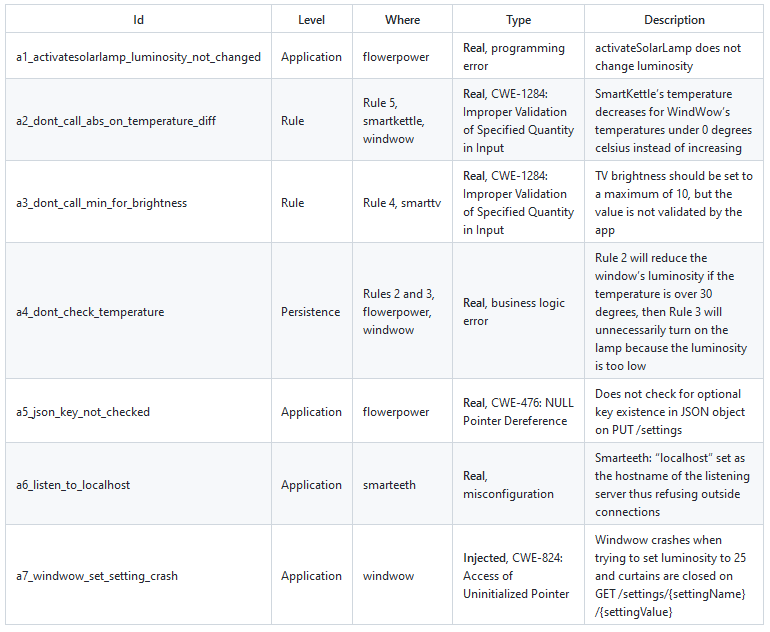
\includegraphics[width=0.9\textwidth]{images/tabel_bug2.png}
    \label{fig:tabel_bug1}
\end{figure}

\begin{figure}[h]
    \centering
    \caption{\centering Lista defectelor din suită (B)}
    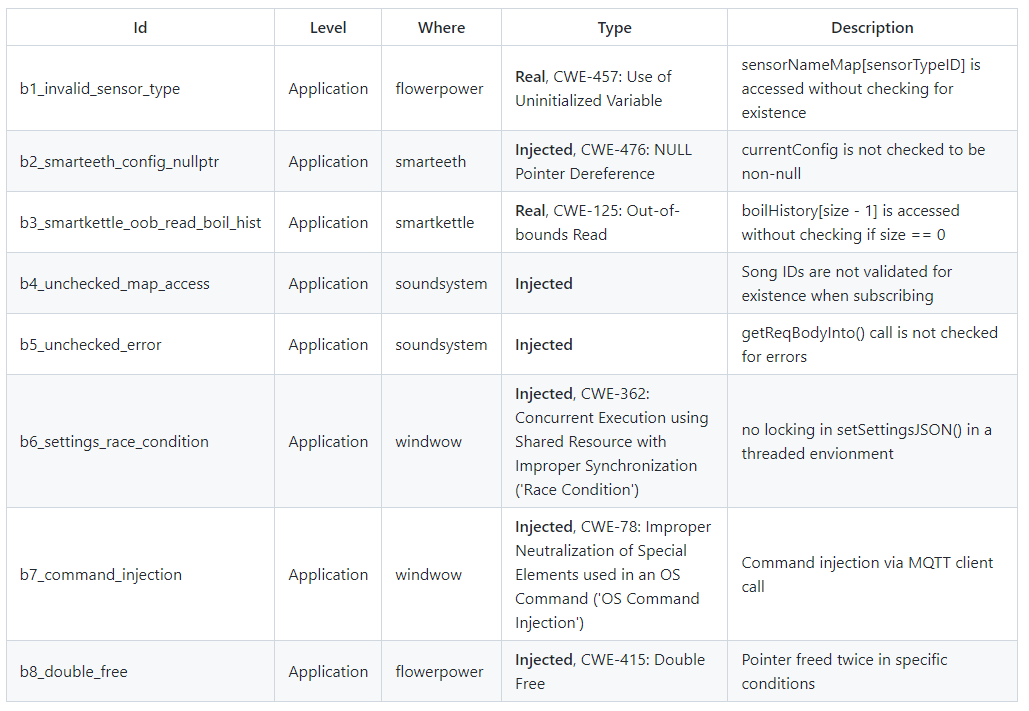
\includegraphics[width=0.9\textwidth]{images/tabel_bug1.png}
    \label{fig:tabel_bug2}
\end{figure}

\chapter{Ilustrații suplimentare}
\label{apx:ilustratii}

\begin{figure}[h]
    \centering
    \caption{\centering Modelul conceptual Open Systems Interconnection \newline (imagine prealuată de pe Wikipedia)}
    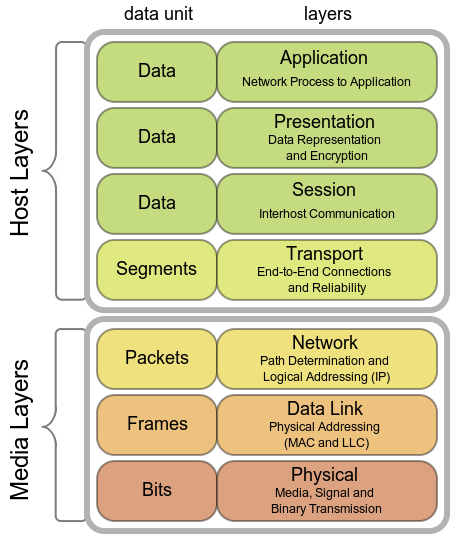
\includegraphics[width=0.8\textwidth]{images/OSI_Model_v1.png}
    \label{fig:osi_model}
\end{figure}

\begin{figure}[h]
    \centering
    \caption{Exemple de topologii ZigBee}
    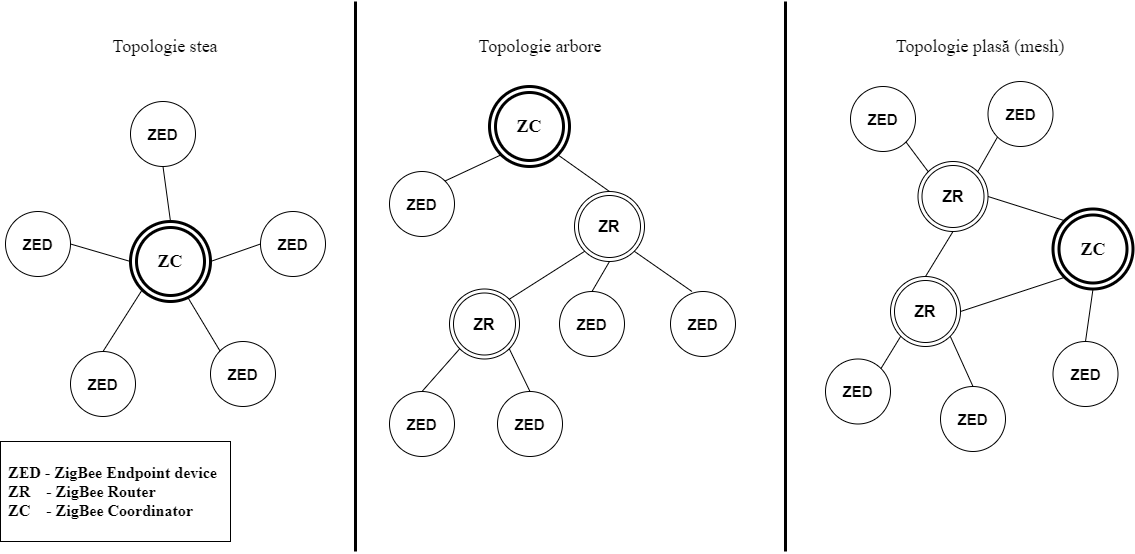
\includegraphics[width=0.9\textwidth]{images/topologii.drawio.png}
    \label{fig:zigbee_networks}
\end{figure}

\begin{landscape}
% Please add the following required packages to your document preamble:
% \usepackage{graphicx}
% \usepackage[table,xcdraw]{xcolor}
% If you use beamer only pass "xcolor=table" option, i.e. \documentclass[xcolor=table]{beamer}
\begin{table}[]
\centering
\resizebox{25cm}{!}{%
\begin{tabular}{|c|c|c|c|c|c|}
\hline
\rowcolor[HTML]{C0C0C0} 
\textbf{Tehnica de testare} &
  \textbf{Grad automatizare} &
  \textbf{Complexitate} &
  \textbf{Niveluri defecte} &
  \textbf{\begin{tabular}[c]{@{}c@{}}Procentaj defecte (cunoscute) detectate\\ (relativ la nivelurile relevante)\end{tabular}} &
  \textbf{Observații} \\ \hline
Testare funcțională BDD &
  Manual &
  Scăzută &
  Toate &
  Nu este relevant &
  \begin{tabular}[c]{@{}c@{}}Componentă exploratorie\\ insuficientă, bun pentru\\ scenarii pozitive\end{tabular} \\ \hline
Fuzzing cu RESTler &
  Automat &
  Medie &
  Aplicație, flux &
  TODO: ??? &
  \begin{tabular}[c]{@{}c@{}}Lipsa înțelegerii stării\\ aplicației, potrivit pentru\\ defecte de logică\end{tabular} \\ \hline
Analiză statică cu weggli &
  Parțial automat &
  Medie &
  Aplicație &
  ??? &
  \begin{tabular}[c]{@{}c@{}}Potrivit pentru defecte\\ de memorie\end{tabular} \\ \hline
Analiză statică cu cppcheck &
  Parțial automat &
  Scăzută &
  Aplicație &
  ??? &
  Rată mare de fals-pozitive \\ \hline
Verificare formală cu TLA+ &
  Parțial automat &
  Ridicată &
  Persistență &
  100\% &
  \begin{tabular}[c]{@{}c@{}}Potrivit pentru defecte\\ de concurență, necesită\\ cunoștințe matematice\end{tabular} \\ \hline
\end{tabular}%
}
\caption{Sumar comparativ al tehnicilor de testare abordate}
\label{tab:sumar_testare}
\end{table}
\end{landscape}

\chapter{Cod sursă suplimentar}
\label{apx:cod}

\begin{lstlisting}[caption={Specificația TLA+ a scenariului descris în capitolul 5, secțiunea despre verificare formală}, label={lst:tla_exemplu}]
----- MODULE light_example -----
EXTENDS Naturals, TLC

LightStates == {"on", "off"}
MotionStates == {"detected", "not detected"}
IsMidnight(x) == IF x % 5 = 0 THEN TRUE ELSE FALSE

\(\* --algorithm light\_example
variables 
    light\_state = "off", 
    motion\_state = "not detected",
    now = 1;

process motion\_sensor = 1
begin
A:
    while TRUE do
        with c\_state \in MotionStates do
            motion\_state := c\_state;
     
            if c\_state = "detected" then
                light\_state := "on";
            end if;
        end with;
    end while;
end process

process clock = 2
begin
B:
    while TRUE do
        now := now + 1;
    end while;
end process

process light\_timer = 3
begin
C:
    while TRUE do
        if IsMidnight(now) then
            light\_state := "off";
        end if;
    end while;
end process

end algorithm; *)
\* BEGIN TRANSLATION 
VARIABLES light\_state, motion\_state, now

vars == << light\_state, motion\_state, now >>

ProcSet == {1} \cup {2} \cup {3}

Init == \(\* Global variables *)
        /\ light\_state = "off"
        /\ motion\_state = "not detected"
        /\ now = 1

motion\_sensor == /\ \E c\_state \in MotionStates:
                      /\ motion\_state' = c\_state
                      /\ IF c\_state = "detected"
                            THEN /\ light\_state' = "on"
                            ELSE /\ TRUE
                                 /\ UNCHANGED light\_state
                 /\ now' = now

clock == /\ now' = now + 1
         /\ UNCHANGED << light\_state, motion\_state >>

light\_timer == /\ IF IsMidnight(now)
                     THEN /\ light\_state' = "off"
                     ELSE /\ TRUE
                          /\ UNCHANGED light\_state
               /\ UNCHANGED << motion\_state, now >>

Next == motion\_sensor \/ clock \/ light\_timer

Spec == Init /\ [][Next]\_vars

\* END TRANSLATION 

MotionLightValid == (motion\_state = "detected") => (light\_state = "on")

=========
\end{lstlisting}

\end{appendices}

\end{document}